\documentclass[../main.tex]{subfiles}
\graphicspath{{\subfix{../images/}}}
\begin{document}

\chapter{MARCO METODOLÓGICO}

%Esta sección describe la propuesta metodológica. La metodología debe ser clara y debe tener un orden lógico. Ella debe tener relación con la problemática y los objetivos propuestos en la sub-sección Objetivos. Se debe tener en cuidado con los términos utilizados en esta sección. Ellos deberían haber sido descritos en el Marco Teórico. En esta parte también es usual colocar un diagrama o esquema que muestre el proceso que seguirán. Recuerde que todo lo expresado aquí debe tener el próposito de ser completamente reproducido por el lector.

\section{Creación del dataset}
\subsection{Dump de Wikipedia en español}

El primer paso para crear el dataset es descargar todo el contenido de Wikipedia en español desde \url{https://dumps.wikimedia.org/eswiki/latest/eswiki-latest-pages-articles.xml.bz2}.

\subsection{Corpus}
Luego convertimos el archivo en un corpus con el siguiente script:
% https://www.kdnuggets.com/2017/11/building-wikipedia-text-corpus-nlp.html
\inputminted[bgcolor=codeBack, tabsize=2]{python}{make_wiki_corpus.py}
\begin{minted}[bgcolor=codeBack, tabsize=2]{bash}
$ ./make_wiki_corpus.py eswiki-latest-pages-articles.xml.bz2 eswiki.txt
\end{minted}

El resultado es \texttt{eswiki.txt}, un archivo corpus.
El cual será un input de Synthdog, la misma herramienta descrita por \citet{kim2022ocrfree}, para la creación de imágenes sintéticas en español.

\subsection{Synthdog}

El último paso para generar las 500.000 imágenes es ejecutar los siguientes comandos en la carpeta \texttt{synthdog} del repositorio de Donut\cite{kim2022ocrfree}.
Al final, en la carpeta \texttt{outputs} estará nuestro dataset \texttt{SynthDoG\_es}
conformado por imágenes y sus metadatos.

\begin{minted}[bgcolor=codeBack, tabsize=2]{bash}
sed "s/enwiki.txt/eswiki.txt/" config_en.yaml > config_es.yaml
mv eswiki.txt resources/corpus/
synthtiger \
	--output ./outputs/SynthDoG_es \
	--count 500000 \
	--worker $(nproc) \
	--verbose \
	template.py \
	SynthDoG \
	config_es.yaml
\end{minted}

\begin{figure}[H]
	\centering
	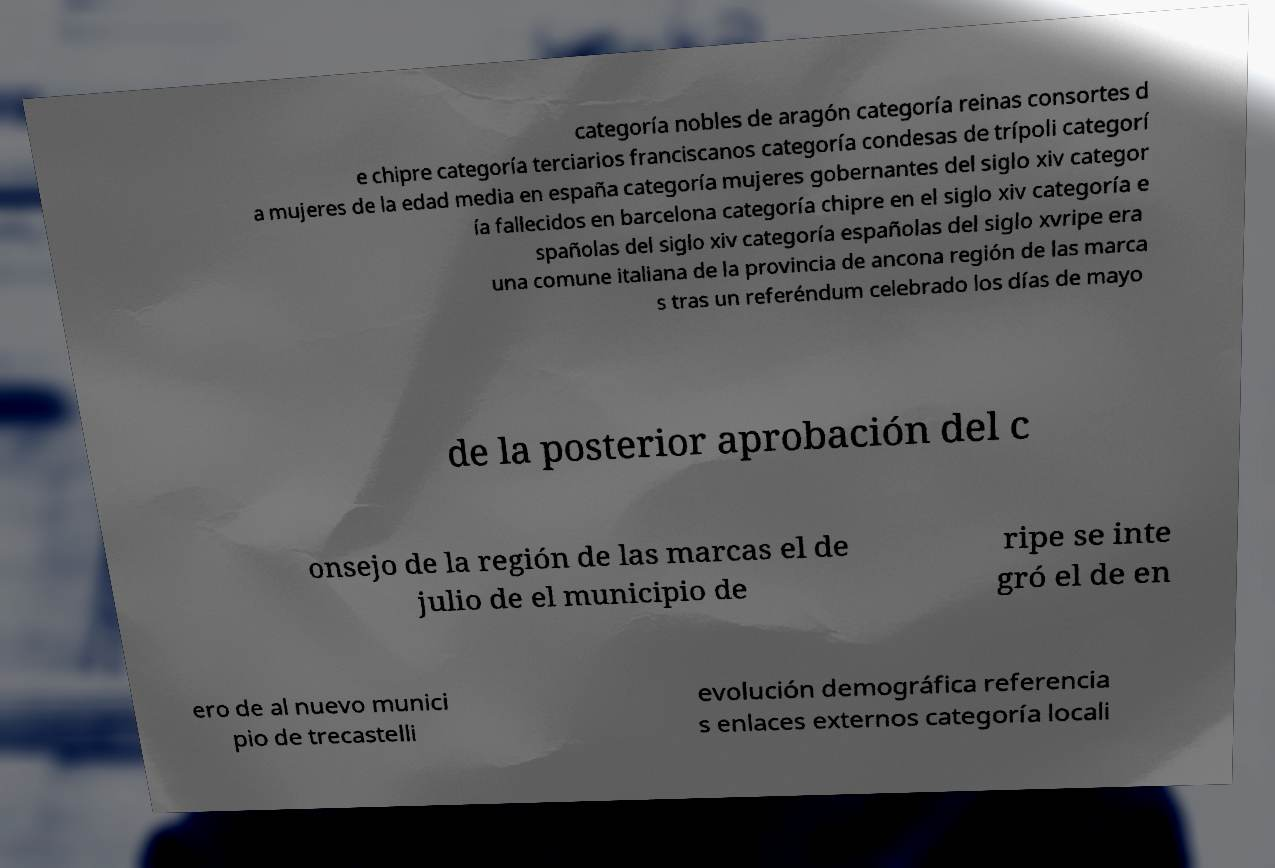
\includegraphics[width=0.9\textwidth]{image_475821.jpg}
	\caption{Ejemplo de imágen generada con SynthDoG}
	%\label{fig:}
\end{figure}

\section{Pre-entrenamiento}

Para hacer que Donut pueda leer documentos en español
lo entrenamos con el dataset previamente creado.
El entrenamiento fue hecho en un GPU Nvidia Ampere A100 (40 GB) del cluster Khipu de UTEC con un batch size de 2.

\inputminted[bgcolor=codeBack, tabsize=2]{bash}{train-es.sh}

\section{Documentos sintéticos}
El dataset del segundo entrenamiento está conformado por 120000 documentos sintéticos generados con DocSim\cite{DocSim} y sus respectivas preguntas y respuestas.

\begin{figure}[H]
	\centering
	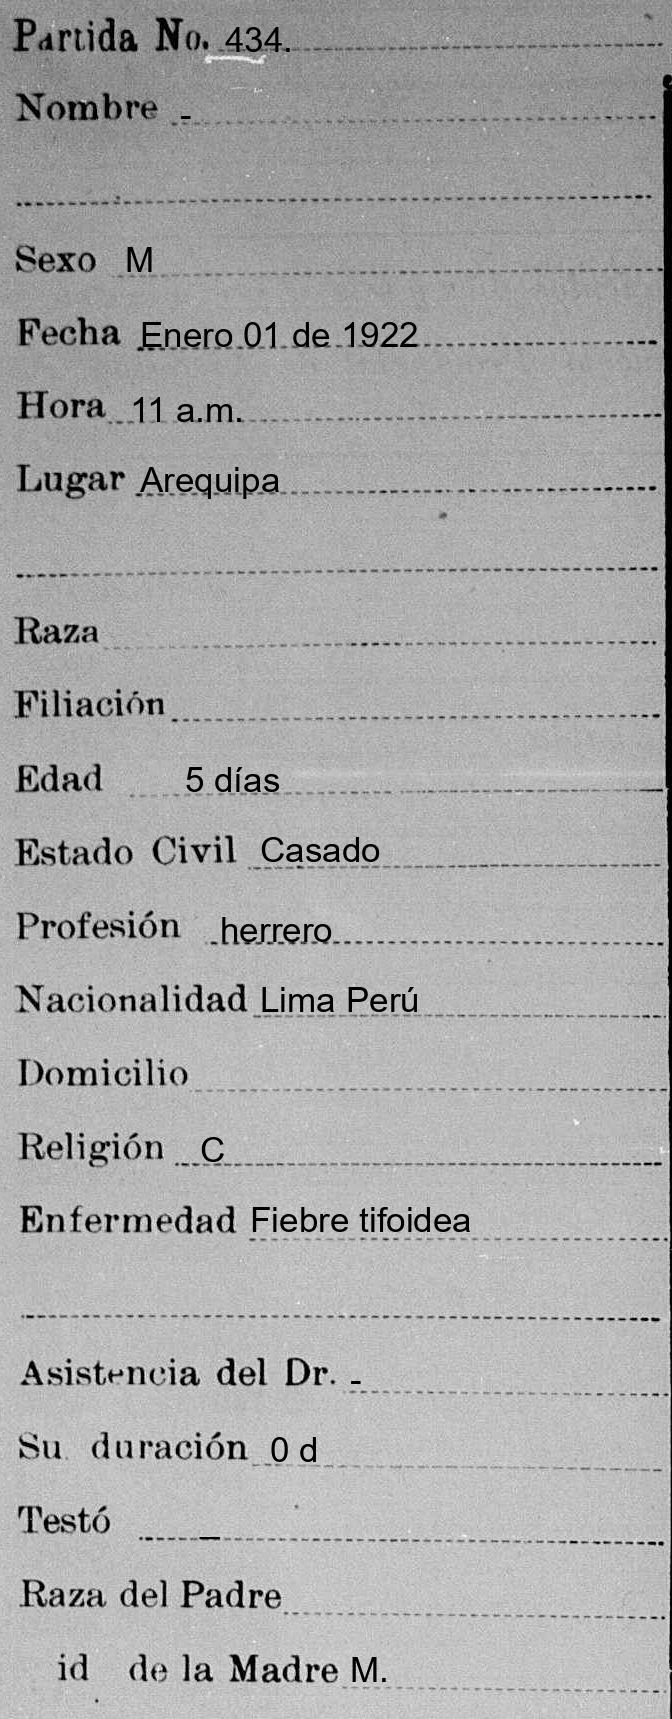
\includegraphics[width=0.25\textwidth]{006cc6cd159e46b5bf3c44c9545fbb25.jpg}
	\caption{Ejemplo de imágen generada con DocSim}
	%\label{fig:}
\end{figure}


\section{Fine tuning}

El último paso para que Donut pueda resolver preguntas de nuestros documentos escaneados es volverlo a entrenar con el dataset sintético. Fue hecho en el mismo hardware con la misma configuración excepto el batch size, el cual fue de 4.

\inputminted[bgcolor=codeBack, tabsize=2]{bash}{train-es-finetuned.sh}

\end{document}
